
\begin{subfigure}{\textwidth}
\centering
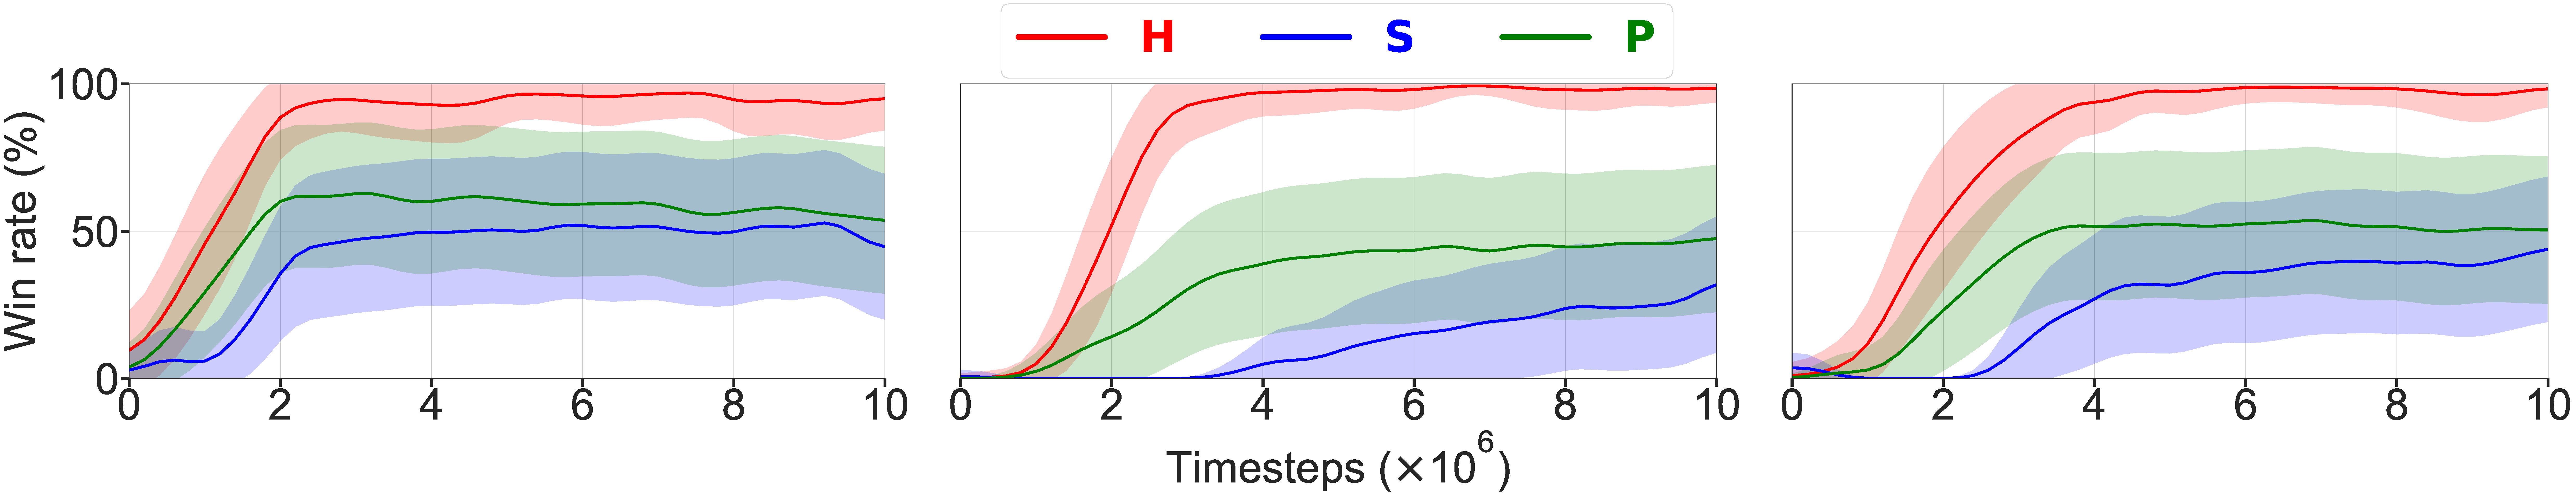
\includegraphics[width=.9\textwidth]{tex_thesis/figures/ch7/tiny_heuristic_plot_qvmixmavenqmix.pdf}
    \begin{subfigure}{.05\textwidth}
    \centering
    \caption*{}
    \end{subfigure}%
    \begin{subfigure}{.31\textwidth}
    \renewcommand\thesubfigure{\alph{subfigure}.1}
      \centering
      \caption{QVMix}
      \label{subfig:vs_h_methodQVMIX}
    \end{subfigure}%
    \begin{subfigure}{.31\textwidth}
    \addtocounter{subfigure}{-1}
    \renewcommand\thesubfigure{\alph{subfigure}.2}
      \centering
      \caption{MAVEN}
      \label{subfig:vs_h_methodMAVEN}
    \end{subfigure}%
    \begin{subfigure}{.31\textwidth}
    \addtocounter{subfigure}{-1}
    \renewcommand\thesubfigure{\alph{subfigure}.3}
      \centering
      \caption{QMIX}
      \label{subfig:vs_h_methodQMIX}
    \end{subfigure}
\addtocounter{subfigure}{-1}
\caption{Win rates achieved against the heuristic in the $3m$ map.}    
\label{subfig:3m_vs_h}
\end{subfigure}
\begin{subfigure}{\textwidth}
    \centering
    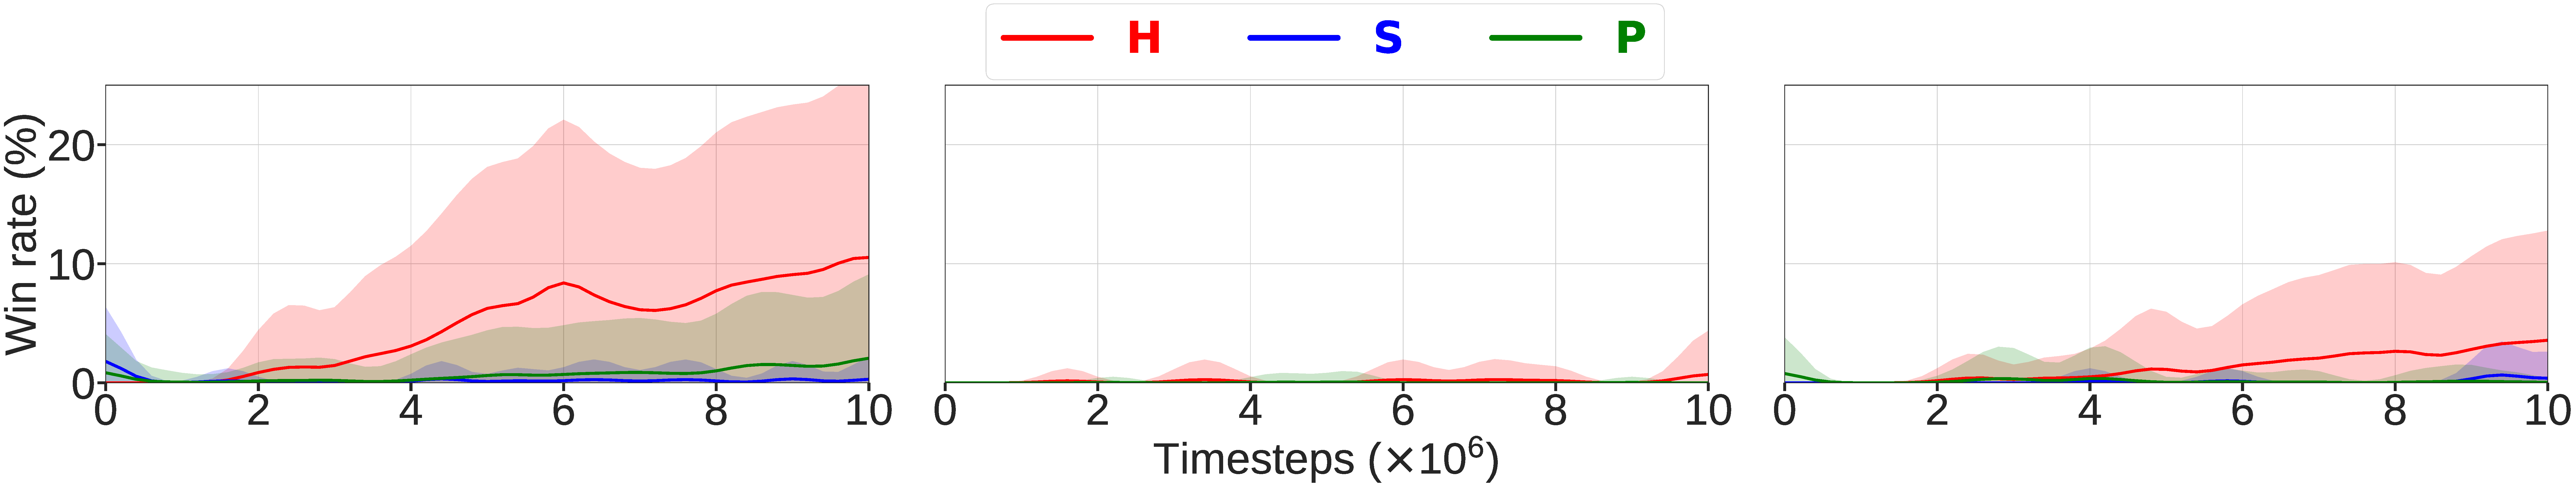
\includegraphics[width=.9\textwidth]{tex_thesis/figures/ch7/3s5z_tiny_heuristic_plot_qvmixmavenqmix.pdf}
    \begin{subfigure}{.05\textwidth}
    \centering
    \caption*{}
    \end{subfigure}%
    \begin{subfigure}{.31\textwidth}
    \renewcommand\thesubfigure{\alph{subfigure}.1}
      \centering
      \caption{QVMix}
      \label{subfig:3s5z_vs_h_methodQVMIX}
    \end{subfigure}%
    \begin{subfigure}{.31\textwidth}
    \addtocounter{subfigure}{-1}
    \renewcommand\thesubfigure{\alph{subfigure}.2}
      \centering
      \caption{MAVEN}
      \label{subfig:3s5z_vs_h_methodMAVEN}
    \end{subfigure}%
    \begin{subfigure}{.31\textwidth}
    \addtocounter{subfigure}{-1}
    \renewcommand\thesubfigure{\alph{subfigure}.3}
      \centering
      \caption{QMIX}
      \label{subfig:3s5z_vs_h_methodQMIX}
    \end{subfigure}
\addtocounter{subfigure}{-1}
\caption{Win rates achieved against the heuristic in the $3s5z$ map. Note the change in scale of the y-axis.}
\label{subfig:3s5z_vsh}
\end{subfigure}
\begin{subfigure}{\textwidth}
\centering
    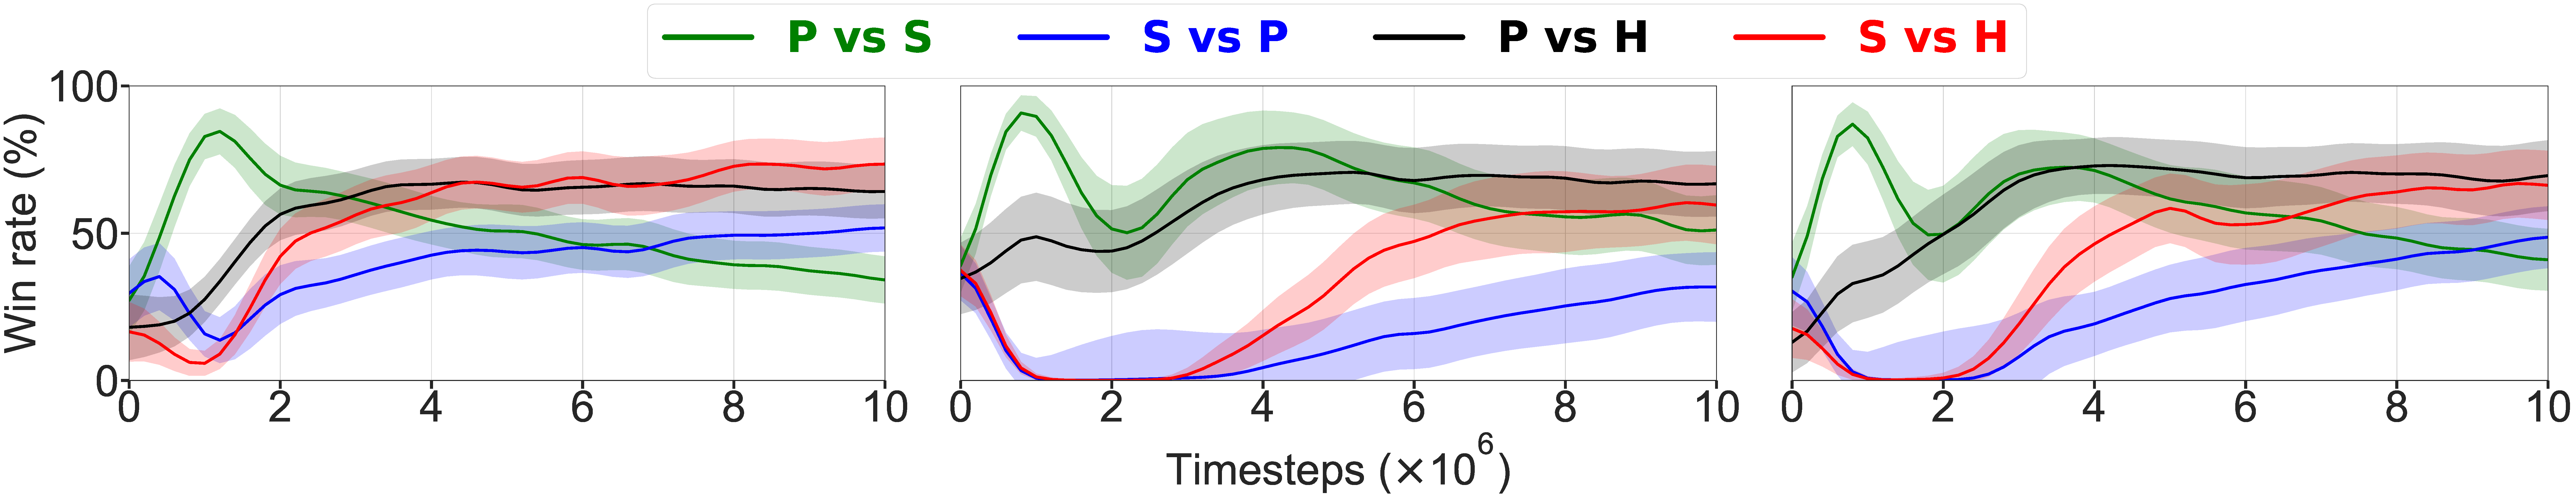
\includegraphics[width=.9\textwidth]{tex_thesis/figures/ch7/tiny_perf_self_popu.pdf}
    \begin{subfigure}{.05\textwidth}
    \centering
    \caption*{}
    \end{subfigure}%
    \begin{subfigure}{.31\textwidth}
    \renewcommand\thesubfigure{\alph{subfigure}.1}
      \centering
      \caption{QVMix}
      \label{subfig:duo_methodQVMIX}
    \end{subfigure}%
    \begin{subfigure}{.31\textwidth}
    \addtocounter{subfigure}{-1}
    \renewcommand\thesubfigure{\alph{subfigure}.2}
      \centering
      \caption{MAVEN}
      \label{subfig:duo_methodMAVEN}
    \end{subfigure}%
    \begin{subfigure}{.31\textwidth}
    \addtocounter{subfigure}{-1}
    \renewcommand\thesubfigure{\alph{subfigure}.3}
      \centering
      \caption{QMIX}
      \label{subfig:duo_methodQMIX}
    \end{subfigure}
\addtocounter{subfigure}{-1}
\caption{Win rates achieved by teams trained in the $3m$ map against themselves.}
\label{subfig:3m_duo}
\end{subfigure}
\begin{subfigure}{\textwidth}
\centering
    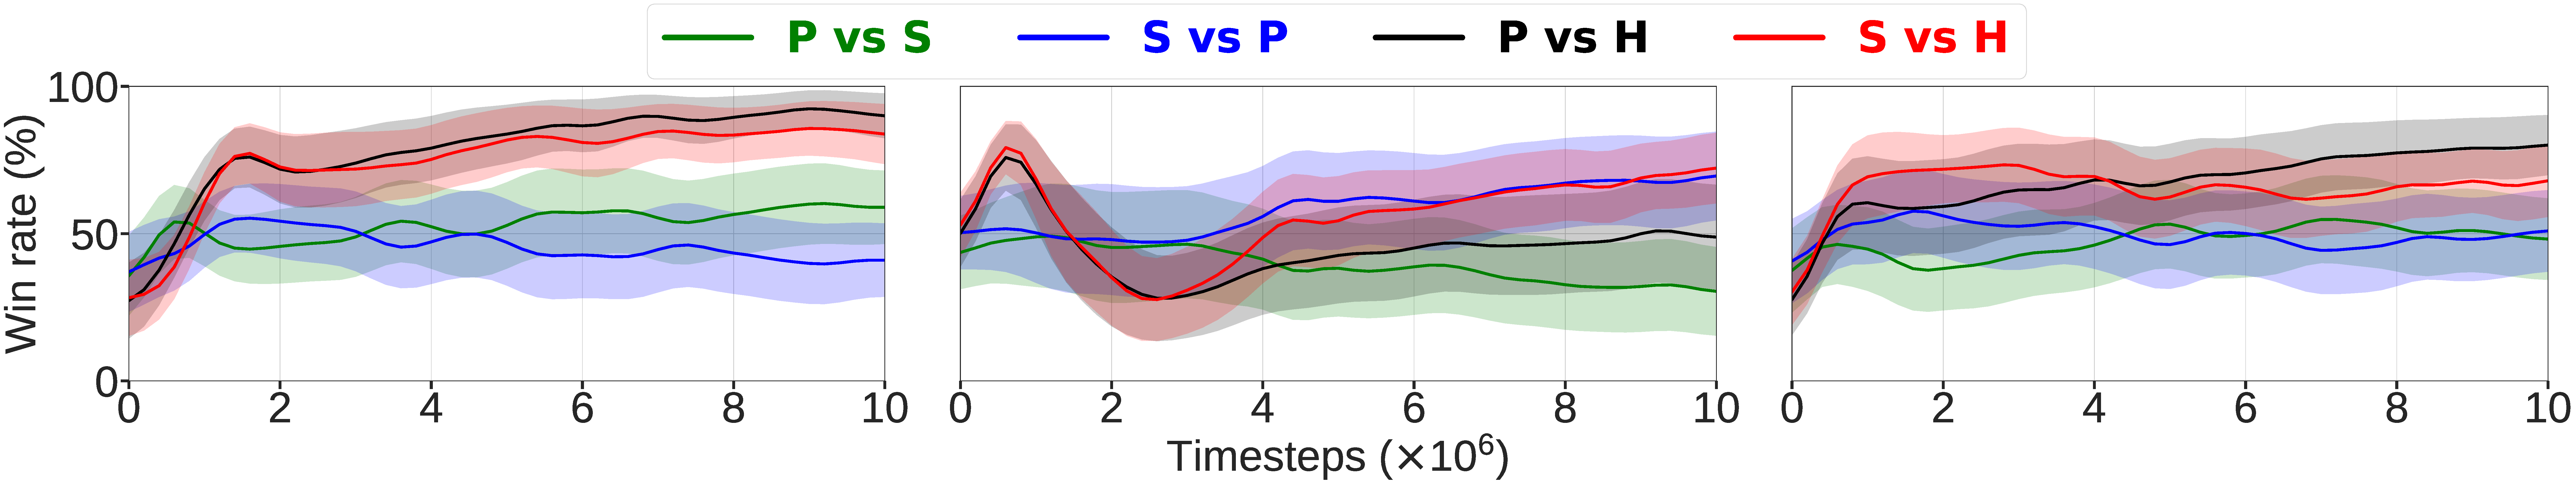
\includegraphics[width=.9\textwidth]{tex_thesis/figures/ch7/3s5z_tiny_perf_self_popu.pdf}
    \begin{subfigure}{.05\textwidth}
    \centering
    \caption*{}
    \end{subfigure}%
    \begin{subfigure}{.31\textwidth}
    \renewcommand\thesubfigure{\alph{subfigure}.1}
      \centering
      \caption{QVMix}
      \label{subfig:3s5z_duo_methodQVMIX}
    \end{subfigure}%
    \begin{subfigure}{.31\textwidth}
    \addtocounter{subfigure}{-1}
    \renewcommand\thesubfigure{\alph{subfigure}.2}
      \centering
      \caption{MAVEN}
      \label{subfig:3s5z_duo_methodMAVEN}
    \end{subfigure}%
    \begin{subfigure}{.31\textwidth}
    \addtocounter{subfigure}{-1}
    \renewcommand\thesubfigure{\alph{subfigure}.3}
      \centering
      \caption{QMIX}
      \label{subfig:3s5z_duo_methodQMIX}
    \end{subfigure}
\addtocounter{subfigure}{-1}
\caption{Win rates achieved by teams trained in the $3s5z$ map against themselves.}
\label{subfig:3s5z_duo}
\end{subfigure}

\caption{
Means of win rate achieved along training time steps by confronting teams trained with the same method against the heuristic or against other teams trained with a different learning scenario.
Teams are trained either with QVMix, MAVEN, or QMIX.
Tests were performed in the $3m$ map, shown at the top, and in the $3s5z$ maps, shown at the bottom. 
Win rates against the heuristic are presented in red, blue and green for teams trained against the heuristic, in self-play and within a population, respectively.
Win rates of teams trained within a population against teams trained in self-play are presented in green and against teams trained against the heuristic in black.
Win rates of teams trained in self-play against teams trained within a population are presented in blue and against teams trained against the heuristic in red.
The error band is half the standard deviation.
} 
\label{fig:heuristic_plot}